\documentclass[a4paper,12pt]{article}
\usepackage[utf8]{inputenc}
\usepackage{ibcat5ia}
\usepackage{opencolor}
\usepackage[toc,page]{appendix}
\usepackage{listings}
%\usepackage{pdfpages}
%\usepackage{subfig}
%\usepackage{minted}
%\usepackage{subcaption} 
%\usepackage{soul}
\usepackage{float}
%\usepackage{graphicx}
\usepackage{pgfplots}
\usepackage[english]{babel}
\usepackage{svg}
\usepackage{amsmath}
\usepackage{mathtools}

\title{Resumen Q1}
\author{Sergio Gómez Damas}
\date{Noviembre 2020}

\begin{document}

\maketitle
\newpage
\tableofcontents
\newpage
\section{Álgebra y Geometría}
\newpage
\section{Cálculo}
\newpage
\section{Empresa}
\newpage
\section{Fundamentos Física}
\newpage
\section{Electrónica en las Telecomunicaciones}
\newpage
\section{Química}
\subsection{Tema 1}
\subsubsection{Identificador del átomo}
\begin{equation}
    ^A_Z X
\end{equation}
\begin{itemize}
    \item \emph{X}: símbolo elemento
    \item \emph{Z}: numero atómico (nº protones)$\Rightarrow$ establece elemento
    \item \emph{A}: numero másico (nº protones +nº neutrones)$\Rightarrow$ establece isótopo
\end{itemize}
\subsubsection{Masa atomica}
\begin{equation}
    m_a=\sum^{n}_{i=1}m_ia_i=m_1a_1+m_2a_2+\dots+m_na_n
\end{equation}
Donde $m_i$ es la masa del isotopo i y $a_i$ su abundancia relativa
\subsubsection{Mol}
\begin{equation}
    N_a=6.022\cdot10^{23}
\end{equation}
\subsubsection{Estados materia}
\begin{figure}[H]
    \centering
    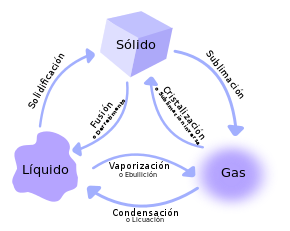
\includegraphics{Imagenes/QUIM/290px-Estados.png}
    \caption{Estados materia}
    \label{fig:estadosmateria}
\end{figure}
\emph{Liquido$\Rightarrow$Gas}:$T<T_{\text{ebullición}}\Rightarrow$evaporación
\begin{figure}[H]
    \centering
    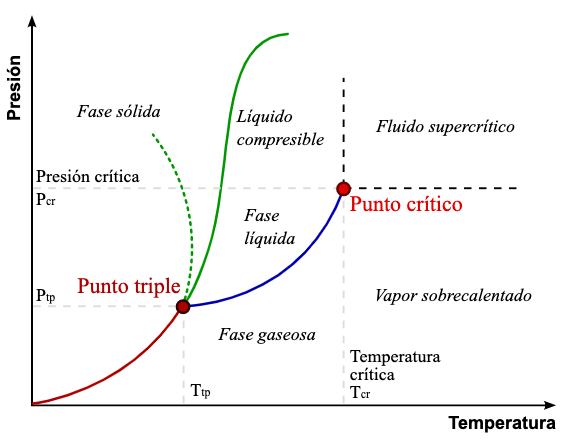
\includegraphics[width=\textwidth]{Imagenes/QUIM/Phase-diag_es.png}
    \caption{Diagrama fase}
\end{figure}
\subsubsection{Disoluciones}
\begin{itemize}
    \item \emph{Soluto}: componente minoritario
    \item \emph{Disolvente}: componente mayoritario
\end{itemize}
\paragraph{Unidades concentración}
\begin{gather}     
    \%\text{masa}=\frac{\text{g soluto}}{\text{g disolución}}\cdot100\\
    \%\text{vol}=\frac{\text{mL soluto}}{\text{mL solución}}\cdot100\\
    \%=\frac{\text{g soluto}}{\text{100mL solución}}\\
    M=\frac{\text{moles soluto}}{\text{L disolución}}\\
    m=\frac{\text{moles soluto}}{\text{Kg disolución}}\\
    \text{fracción molar X}=\frac{\text{moles soluto}}{\text{moles soluto}+\text{moles dissolvente}}
\end{gather}
\subsection{Tema 2}
\end{document}

